% @author Marcel Ruland (2018)
\documentclass{article}
\usepackage{tikz}
\usetikzlibrary{positioning}
\usetikzlibrary{arrows}
\renewcommand{\familydefault}{\sfdefault}
\begin{document}
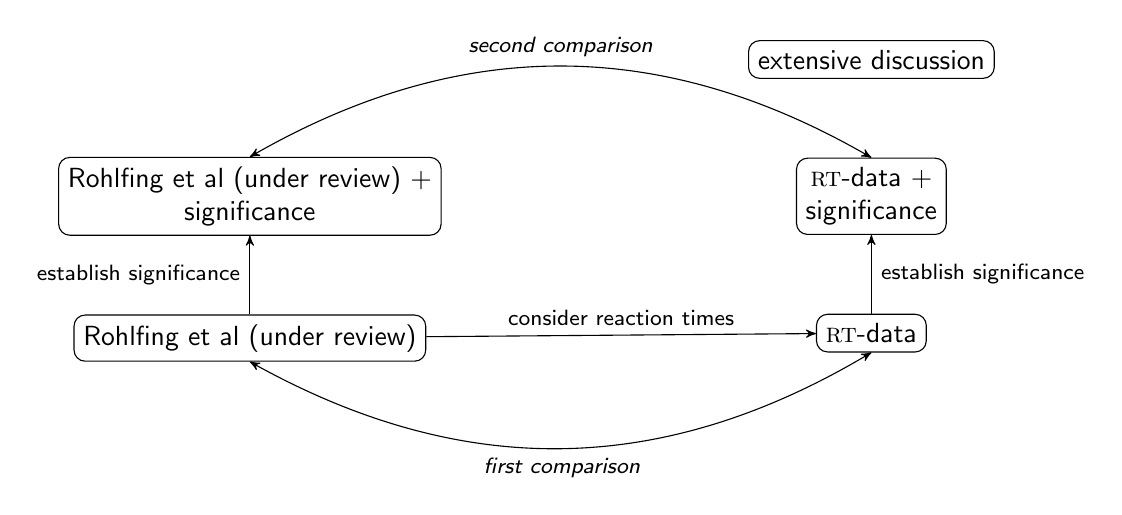
\begin{tikzpicture}
	[%every node/.append style={font=\sffamily\addfontfeature{Numbers=Lining}},
	node distance=1cm and 4.5cm,
	rounded corners,
	align=center,
	>=stealth']
	
	% nodes
	\node [draw] (sig) {Rohlfing et al (under review) + \\ significance};
	\node [draw, right=of sig] (reacsig) {\textsc{rt}-data + \\ significance};
	\node [draw, below=of sig] (origin) {Rohlfing et al (under review)};
	\node [draw, below=of reacsig] (reac) {\textsc{rt}-data};
	\node [draw, above=of reacsig, node distance= 1cm and 1cm] (discuss) {extensive discussion};
	
	% straightarrows
	\draw [->] (origin) -- node[above] {\footnotesize consider reaction times} (reac);
	\draw [->] (origin) -- node[left]  {\footnotesize establish significance}  (sig);
	\draw [->] (reac)   -- node[right] {\footnotesize establish significance}  (reacsig);
	
	% curved arrows
	\draw[<->] (sig.north) to[bend left] node[above]{\footnotesize\textit{second comparison}} (reacsig.north);
	\draw[<->] (origin.south) to[bend right] node[below]{\footnotesize\textit{first comparison}} (reac.south);
\end{tikzpicture}
\end{document}














































